% Graph-worthiness rule. % Graph-worthiness rule. % Graph-worthiness rule. % Graph-worthiness rule. \input{graph_worthiness_section} from main.tex (after the cross-GPU
% results). Numbers: results/graph_worthiness.md (model/graph_worthiness.py).
\subsection{When is a CUDA graph worth capturing?}
\label{sec:graphworthiness}

Capturing a region of a PyTorch policy as a CUDA graph is engineering work: buffers must be
static, host synchronizations removed, constant uploads moved out of the region and every input
kept alive. For SmolVLA the vision encoder could not be captured at all (a data dependent
\texttt{arange}), and for OpenVLA the decoder needed a static KV cache and two library patches.
A practitioner therefore wants to know \emph{before} capturing whether the speedup justifies the
work. We give a rule that answers this from eager mode only.

\paragraph{Rule.}
For a candidate region let $T_e$ be its eager wall time, $K$ its number of kernel launches and
$D$ the summed duration of those kernels in one profiled eager step. We predict
\begin{equation}
  \hat T_g = D + K\varepsilon, \qquad \hat S = \frac{T_e}{D + K\varepsilon}
  \approx \frac{c}{t + \varepsilon},
  \label{eq:graphworthiness}
\end{equation}
where $c = T_e/K$ is the eager time per kernel (mostly host dispatch), $t = D/K$ the mean traced
kernel time and $\varepsilon$ the net per-kernel cost of a graph node relative to a traced eager
duration. $\varepsilon$ is the graph node cost minus the profiler's bias on each traced kernel,
so it can be negative. A region is worth capturing when $\hat S$ exceeds a threshold. No graph is
captured to make the prediction.

\paragraph{Evaluation.}
We apply the rule to every run for which we have both an eager kernel trace and a measured graph
time of the same region: SmolVLA (camera, step, chunk, batch and RoboTwin variants), SmolVLA
under \texttt{torch.compile} (fused Triton kernels, eager launches vs.\ compile plus CUDA graph),
$\pi_0$, $\pi_{0.5}$, ACT, Diffusion Policy (default and autotuned cuDNN) and the autoregressive
decoders OpenVLA-7B and $\pi_0$-FAST. That is 114 runs, 95 distinct (configuration, GPU)
situations, 8 policies and 4 GPUs, with measured speedups from 0.99$\times$ to 24.3$\times$. The
SmolVLA baseline configuration, which the fitted variants use, is excluded on every GPU. Repeat
runs make the runs partly dependent, so we also report errors per situation and 95\% confidence
intervals from a bootstrap that resamples configurations. We compare five ways to obtain
$\varepsilon$ that use progressively less information about the predicted run, and two baselines
that need no $\varepsilon$ (Table~\ref{tab:graphworthiness}).

\begin{table*}[t]
\centering
\caption{Error of the predicted CUDA-graph speedup (MAPE over 114 held-out runs, 95\% bootstrap
CI over configurations) and decision accuracy at a 10$\times$ threshold, overall and on the 23
runs whose measured speedup lies within a factor 1.25 of it.}
\label{tab:graphworthiness}
\small
\begin{tabular}{llrrr}
\toprule
Variant & $\varepsilon$ from & MAPE & 95\% CI & 10$\times$ decision (all / hard) \\
\midrule
one $\varepsilon$        & one 2080 Ti run          & 7.1\%  & 4.6--9.9   & 92\% / 61\% \\
$\varepsilon$ per GPU    & one SmolVLA run per GPU  & 1.8\%  & 1.0--2.8   & 98\% / 91\% \\
leave policy out         & other policies, same GPU & 2.5\%  & 1.5--3.8   & 98\% / 91\% \\
leave GPU out            & other GPUs only          & 12.7\% & 8.6--17.1  & 91\% / 57\% \\
\midrule
$T_e/D$ (no $\varepsilon$) & none                   & 7.1\%  & 4.6--9.7   & 98\% / 91\% \\
$1/\text{GPU busy}$      & none (utilization)       & 16.9\% & 11.0--23.7 & 89\% / 57\% \\
\bottomrule
\end{tabular}
\end{table*}

\paragraph{Results.}
With $\varepsilon$ calibrated once per GPU the rule predicts the speedup within 1.8\% on average
(1.9\%, 2.7\%, 1.8\% and 1.1\% on the 2080 Ti, A100, RTX 4070 and TITAN V), and within 2.5\% when
$\varepsilon$ comes only from \emph{other} policies on the same GPU, so a value measured on one
workload transfers to unseen ones, including fused \texttt{torch.compile} kernels (3.1\%) and
autoregressive decoders (OpenVLA 3.6\%, $\pi_0$-FAST 2.1\%). Figure~\ref{fig:graphworthiness}
shows the predictions. The fitted values ($+0.52$, $-0.65$, $-0.35$ and $+0.80\,\mu$s) follow
$\varepsilon = \delta_\text{node} - b$: with the node cost $\delta_\text{node}$ from our C++
calibration and the profiler bias $b$ fitted independently by the cross-GPU model
(Section~\ref{sec:crossgpu}), $\delta_\text{node} - b$ is $+0.43$, $-0.71$ and $+0.69\,\mu$s on
the 2080 Ti, A100 and TITAN V. $\varepsilon$ does not transfer across machines (leave GPU out,
12.7\%) because $b$ is a property of each host's profiler. A utilization counter is a poor
substitute: $1/\text{busy}$ is 16.9\% off and up to 62\% for single runs, because the busy
fraction of a whole step mixes the captured region with the parts that stay eager.

The decision is what a practitioner needs. Most regions are far from a 1.5$\times$ threshold, so
every predictor except the utilization baseline is right for all runs there. We therefore score
decisions at 25 thresholds from 1.2$\times$ to 15$\times$ and separately on the hard runs near
each threshold (Figure~\ref{fig:graphworthiness_threshold}). The leave-policy-out rule is right
for at least 94\% of the runs at every threshold and for 91\% of the hard runs at 5$\times$ and
10$\times$; dropping $\varepsilon$ gives 55\% of the hard runs at 5$\times$, and the utilization
baseline is wrong for up to 18\% of all runs. Within each GPU the predicted speedups order the
regions almost exactly (Spearman $\rho \ge 0.973$).

\paragraph{What sets the speedup.}
Across all eight policies the eager time per kernel $c$ stays between 26 and $44\,\mu$s, while
the mean kernel time $t$ ranges from $3.7\,\mu$s (SmolVLA) to $41\,\mu$s (Diffusion Policy). By
Eq.~\ref{eq:graphworthiness} the speedup is set mainly by $t$: SmolVLA, $\pi_0$ and $\pi_{0.5}$
($t \approx 4$ to $5\,\mu$s) gain up to 24$\times$ at batch 1, ACT, \texttt{torch.compile} and
the decoders ($t \approx 9$ to $13\,\mu$s) 1.1 to 11$\times$, and Diffusion Policy
($t \approx 41\,\mu$s) gains nothing. Batching moves a region along the same curve: SmolVLA's
loop falls from 10$\times$ at batch 1 to 2.1$\times$ at batch 16 on the 2080 Ti as $t$ grows. The same equation explains the eager/graph inversion across GPUs
(Section~\ref{sec:crossgpu}): a slower host raises $c$, a faster GPU lowers $t$, and both raise
the speedup.

\paragraph{How to profile.}
Two measurement rules matter. First, long profiling sessions inflate CUPTI's traced durations on
two of our hosts: a 20-step SmolVLA profile adds about $1\,\mu$s per kernel on the 2080 Ti and A100
hosts and the rule is then 18 to 25\% off, while $K$ and $D$ from a 5-step profile scaled to 20
steps are within 0.2\%. Profile a short window of a periodic loop. Second, profile on a quiet
host. In our host-contention experiment (one core shared with a CPU hog) a profile taken under
contention inflates $t$ from 3.0 to $4.1\,\mu$s and the rule is 19 to 25\% low for SmolVLA, while
$K$ and $D$ from the quiet run with $T_e$ from the contended run are within $+8\%$. ACT stays 27 to
31\% off under two of the three contention modes because its captured region is the whole step,
including host work that contention slows in graph mode too.

\paragraph{Limitations.}
The decoder windows come from the stock dynamic-cache decoder, which launches about 3\% more
kernels per token than the static-cache path that is graphed; OpenVLA has two runs on one GPU.
$\varepsilon$ needs one calibration run per machine. We also measured it without any policy,
with a microbenchmark (\texttt{workloads/eps\_probe.py}: graph time per kernel minus the
CUPTI-traced eager duration on chains of seven small op types at SmolVLA's shapes). On the 2080 Ti
and RTX 4070 it gives $+0.11$ and $-0.05\,\mu$s against $+0.52$ and $-0.35\,\mu$s fitted from
SmolVLA; over the 66 runs on those two GPUs the rule is then 5.2\% off (CI 3.5--7.2\%), better than
no $\varepsilon$ (6.2\%) or one $\varepsilon$ for all GPUs (7.4\%) but well behind one calibration
run of any policy (1.9\% per GPU, 2.4\% leave policy out). The gap differs in sign between the
GPUs, so it is not a constant offset: kernels inside a real policy run with a different cache
state and clock than hot microbenchmark chains, and the RTX 4070 probe ran under a different
PyTorch build (2.8 vs.\ 2.10, so a different CUPTI) than its traces. We therefore recommend
calibrating $\varepsilon$ on one run of a representative policy. The rule predicts the speedup of a region whose kernels stay the same under capture; it
does not predict what fusion would achieve.

\begin{figure}[t]
\centering
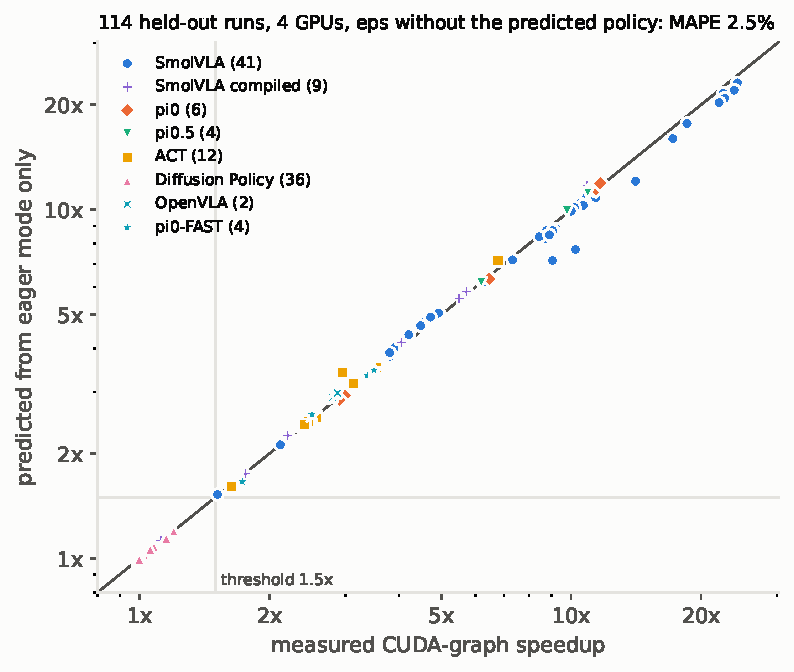
\includegraphics[width=\columnwidth]{figures/graph_worthiness.pdf}
\caption{Graph-worthiness rule: CUDA-graph speedup predicted from eager mode only vs.\ measured,
114 held-out runs on four GPUs, $\varepsilon$ fitted without the predicted policy.}
\label{fig:graphworthiness}
\end{figure}

\begin{figure}[t]
\centering
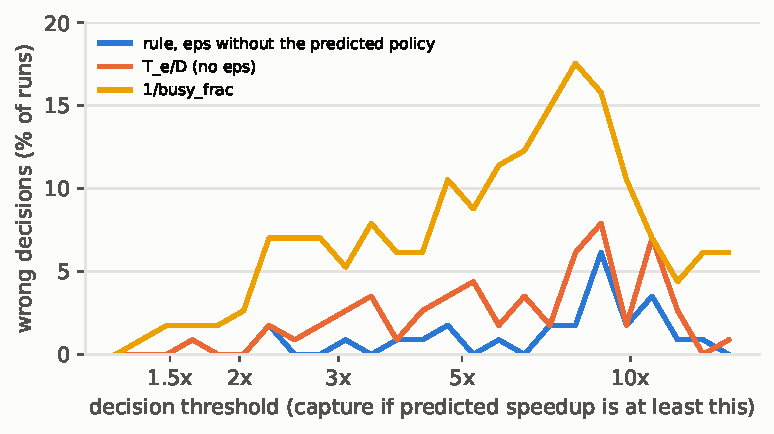
\includegraphics[width=\columnwidth]{figures/graph_worthiness_threshold.pdf}
\caption{Wrong capture decisions as a function of the threshold. Always capturing is wrong for
32 to 93\% of the runs over this range (not shown).}
\label{fig:graphworthiness_threshold}
\end{figure}
 from main.tex (after the cross-GPU
% results). Numbers: results/graph_worthiness.md (model/graph_worthiness.py).
\subsection{When is a CUDA graph worth capturing?}
\label{sec:graphworthiness}

Capturing a region of a PyTorch policy as a CUDA graph is engineering work: buffers must be
static, host synchronizations removed, constant uploads moved out of the region and every input
kept alive. For SmolVLA the vision encoder could not be captured at all (a data dependent
\texttt{arange}), and for OpenVLA the decoder needed a static KV cache and two library patches.
A practitioner therefore wants to know \emph{before} capturing whether the speedup justifies the
work. We give a rule that answers this from eager mode only.

\paragraph{Rule.}
For a candidate region let $T_e$ be its eager wall time, $K$ its number of kernel launches and
$D$ the summed duration of those kernels in one profiled eager step. We predict
\begin{equation}
  \hat T_g = D + K\varepsilon, \qquad \hat S = \frac{T_e}{D + K\varepsilon}
  \approx \frac{c}{t + \varepsilon},
  \label{eq:graphworthiness}
\end{equation}
where $c = T_e/K$ is the eager time per kernel (mostly host dispatch), $t = D/K$ the mean traced
kernel time and $\varepsilon$ the net per-kernel cost of a graph node relative to a traced eager
duration. $\varepsilon$ is the graph node cost minus the profiler's bias on each traced kernel,
so it can be negative. A region is worth capturing when $\hat S$ exceeds a threshold. No graph is
captured to make the prediction.

\paragraph{Evaluation.}
We apply the rule to every run for which we have both an eager kernel trace and a measured graph
time of the same region: SmolVLA (camera, step, chunk, batch and RoboTwin variants), SmolVLA
under \texttt{torch.compile} (fused Triton kernels, eager launches vs.\ compile plus CUDA graph),
$\pi_0$, $\pi_{0.5}$, ACT, Diffusion Policy (default and autotuned cuDNN) and the autoregressive
decoders OpenVLA-7B and $\pi_0$-FAST. That is 114 runs, 95 distinct (configuration, GPU)
situations, 8 policies and 4 GPUs, with measured speedups from 0.99$\times$ to 24.3$\times$. The
SmolVLA baseline configuration, which the fitted variants use, is excluded on every GPU. Repeat
runs make the runs partly dependent, so we also report errors per situation and 95\% confidence
intervals from a bootstrap that resamples configurations. We compare five ways to obtain
$\varepsilon$ that use progressively less information about the predicted run, and two baselines
that need no $\varepsilon$ (Table~\ref{tab:graphworthiness}).

\begin{table*}[t]
\centering
\caption{Error of the predicted CUDA-graph speedup (MAPE over 114 held-out runs, 95\% bootstrap
CI over configurations) and decision accuracy at a 10$\times$ threshold, overall and on the 23
runs whose measured speedup lies within a factor 1.25 of it.}
\label{tab:graphworthiness}
\small
\begin{tabular}{llrrr}
\toprule
Variant & $\varepsilon$ from & MAPE & 95\% CI & 10$\times$ decision (all / hard) \\
\midrule
one $\varepsilon$        & one 2080 Ti run          & 7.1\%  & 4.6--9.9   & 92\% / 61\% \\
$\varepsilon$ per GPU    & one SmolVLA run per GPU  & 1.8\%  & 1.0--2.8   & 98\% / 91\% \\
leave policy out         & other policies, same GPU & 2.5\%  & 1.5--3.8   & 98\% / 91\% \\
leave GPU out            & other GPUs only          & 12.7\% & 8.6--17.1  & 91\% / 57\% \\
\midrule
$T_e/D$ (no $\varepsilon$) & none                   & 7.1\%  & 4.6--9.7   & 98\% / 91\% \\
$1/\text{GPU busy}$      & none (utilization)       & 16.9\% & 11.0--23.7 & 89\% / 57\% \\
\bottomrule
\end{tabular}
\end{table*}

\paragraph{Results.}
With $\varepsilon$ calibrated once per GPU the rule predicts the speedup within 1.8\% on average
(1.9\%, 2.7\%, 1.8\% and 1.1\% on the 2080 Ti, A100, RTX 4070 and TITAN V), and within 2.5\% when
$\varepsilon$ comes only from \emph{other} policies on the same GPU, so a value measured on one
workload transfers to unseen ones, including fused \texttt{torch.compile} kernels (3.1\%) and
autoregressive decoders (OpenVLA 3.6\%, $\pi_0$-FAST 2.1\%). Figure~\ref{fig:graphworthiness}
shows the predictions. The fitted values ($+0.52$, $-0.65$, $-0.35$ and $+0.80\,\mu$s) follow
$\varepsilon = \delta_\text{node} - b$: with the node cost $\delta_\text{node}$ from our C++
calibration and the profiler bias $b$ fitted independently by the cross-GPU model
(Section~\ref{sec:crossgpu}), $\delta_\text{node} - b$ is $+0.43$, $-0.71$ and $+0.69\,\mu$s on
the 2080 Ti, A100 and TITAN V. $\varepsilon$ does not transfer across machines (leave GPU out,
12.7\%) because $b$ is a property of each host's profiler. A utilization counter is a poor
substitute: $1/\text{busy}$ is 16.9\% off and up to 62\% for single runs, because the busy
fraction of a whole step mixes the captured region with the parts that stay eager.

The decision is what a practitioner needs. Most regions are far from a 1.5$\times$ threshold, so
every predictor except the utilization baseline is right for all runs there. We therefore score
decisions at 25 thresholds from 1.2$\times$ to 15$\times$ and separately on the hard runs near
each threshold (Figure~\ref{fig:graphworthiness_threshold}). The leave-policy-out rule is right
for at least 94\% of the runs at every threshold and for 91\% of the hard runs at 5$\times$ and
10$\times$; dropping $\varepsilon$ gives 55\% of the hard runs at 5$\times$, and the utilization
baseline is wrong for up to 18\% of all runs. Within each GPU the predicted speedups order the
regions almost exactly (Spearman $\rho \ge 0.973$).

\paragraph{What sets the speedup.}
Across all eight policies the eager time per kernel $c$ stays between 26 and $44\,\mu$s, while
the mean kernel time $t$ ranges from $3.7\,\mu$s (SmolVLA) to $41\,\mu$s (Diffusion Policy). By
Eq.~\ref{eq:graphworthiness} the speedup is set mainly by $t$: SmolVLA, $\pi_0$ and $\pi_{0.5}$
($t \approx 4$ to $5\,\mu$s) gain up to 24$\times$ at batch 1, ACT, \texttt{torch.compile} and
the decoders ($t \approx 9$ to $13\,\mu$s) 1.1 to 11$\times$, and Diffusion Policy
($t \approx 41\,\mu$s) gains nothing. Batching moves a region along the same curve: SmolVLA's
loop falls from 10$\times$ at batch 1 to 2.1$\times$ at batch 16 on the 2080 Ti as $t$ grows. The same equation explains the eager/graph inversion across GPUs
(Section~\ref{sec:crossgpu}): a slower host raises $c$, a faster GPU lowers $t$, and both raise
the speedup.

\paragraph{How to profile.}
Two measurement rules matter. First, long profiling sessions inflate CUPTI's traced durations on
two of our hosts: a 20-step SmolVLA profile adds about $1\,\mu$s per kernel on the 2080 Ti and A100
hosts and the rule is then 18 to 25\% off, while $K$ and $D$ from a 5-step profile scaled to 20
steps are within 0.2\%. Profile a short window of a periodic loop. Second, profile on a quiet
host. In our host-contention experiment (one core shared with a CPU hog) a profile taken under
contention inflates $t$ from 3.0 to $4.1\,\mu$s and the rule is 19 to 25\% low for SmolVLA, while
$K$ and $D$ from the quiet run with $T_e$ from the contended run are within $+8\%$. ACT stays 27 to
31\% off under two of the three contention modes because its captured region is the whole step,
including host work that contention slows in graph mode too.

\paragraph{Limitations.}
The decoder windows come from the stock dynamic-cache decoder, which launches about 3\% more
kernels per token than the static-cache path that is graphed; OpenVLA has two runs on one GPU.
$\varepsilon$ needs one calibration run per machine. We also measured it without any policy,
with a microbenchmark (\texttt{workloads/eps\_probe.py}: graph time per kernel minus the
CUPTI-traced eager duration on chains of seven small op types at SmolVLA's shapes). On the 2080 Ti
and RTX 4070 it gives $+0.11$ and $-0.05\,\mu$s against $+0.52$ and $-0.35\,\mu$s fitted from
SmolVLA; over the 66 runs on those two GPUs the rule is then 5.2\% off (CI 3.5--7.2\%), better than
no $\varepsilon$ (6.2\%) or one $\varepsilon$ for all GPUs (7.4\%) but well behind one calibration
run of any policy (1.9\% per GPU, 2.4\% leave policy out). The gap differs in sign between the
GPUs, so it is not a constant offset: kernels inside a real policy run with a different cache
state and clock than hot microbenchmark chains, and the RTX 4070 probe ran under a different
PyTorch build (2.8 vs.\ 2.10, so a different CUPTI) than its traces. We therefore recommend
calibrating $\varepsilon$ on one run of a representative policy. The rule predicts the speedup of a region whose kernels stay the same under capture; it
does not predict what fusion would achieve.

\begin{figure}[t]
\centering
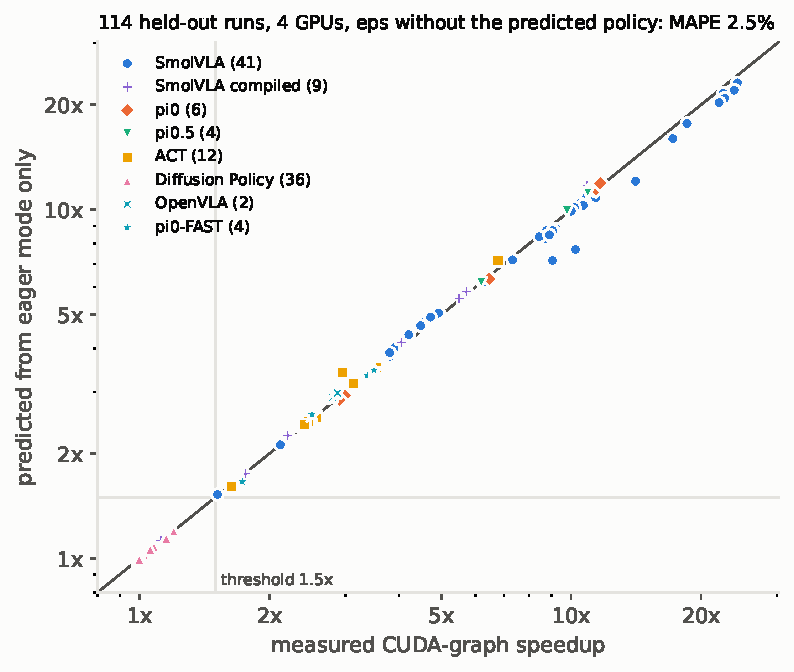
\includegraphics[width=\columnwidth]{figures/graph_worthiness.pdf}
\caption{Graph-worthiness rule: CUDA-graph speedup predicted from eager mode only vs.\ measured,
114 held-out runs on four GPUs, $\varepsilon$ fitted without the predicted policy.}
\label{fig:graphworthiness}
\end{figure}

\begin{figure}[t]
\centering
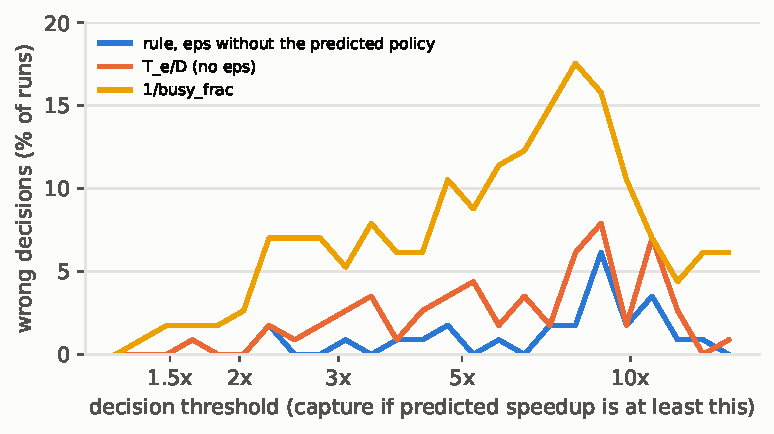
\includegraphics[width=\columnwidth]{figures/graph_worthiness_threshold.pdf}
\caption{Wrong capture decisions as a function of the threshold. Always capturing is wrong for
32 to 93\% of the runs over this range (not shown).}
\label{fig:graphworthiness_threshold}
\end{figure}
 from main.tex (after the cross-GPU
% results). Numbers: results/graph_worthiness.md (model/graph_worthiness.py).
\subsection{When is a CUDA graph worth capturing?}
\label{sec:graphworthiness}

Capturing a region of a PyTorch policy as a CUDA graph is engineering work: buffers must be
static, host synchronizations removed, constant uploads moved out of the region and every input
kept alive. For SmolVLA the vision encoder could not be captured at all (a data dependent
\texttt{arange}), and for OpenVLA the decoder needed a static KV cache and two library patches.
A practitioner therefore wants to know \emph{before} capturing whether the speedup justifies the
work. We give a rule that answers this from eager mode only.

\paragraph{Rule.}
For a candidate region let $T_e$ be its eager wall time, $K$ its number of kernel launches and
$D$ the summed duration of those kernels in one profiled eager step. We predict
\begin{equation}
  \hat T_g = D + K\varepsilon, \qquad \hat S = \frac{T_e}{D + K\varepsilon}
  \approx \frac{c}{t + \varepsilon},
  \label{eq:graphworthiness}
\end{equation}
where $c = T_e/K$ is the eager time per kernel (mostly host dispatch), $t = D/K$ the mean traced
kernel time and $\varepsilon$ the net per-kernel cost of a graph node relative to a traced eager
duration. $\varepsilon$ is the graph node cost minus the profiler's bias on each traced kernel,
so it can be negative. A region is worth capturing when $\hat S$ exceeds a threshold. No graph is
captured to make the prediction.

\paragraph{Evaluation.}
We apply the rule to every run for which we have both an eager kernel trace and a measured graph
time of the same region: SmolVLA (camera, step, chunk, batch and RoboTwin variants), SmolVLA
under \texttt{torch.compile} (fused Triton kernels, eager launches vs.\ compile plus CUDA graph),
$\pi_0$, $\pi_{0.5}$, ACT, Diffusion Policy (default and autotuned cuDNN) and the autoregressive
decoders OpenVLA-7B and $\pi_0$-FAST. That is 114 runs, 95 distinct (configuration, GPU)
situations, 8 policies and 4 GPUs, with measured speedups from 0.99$\times$ to 24.3$\times$. The
SmolVLA baseline configuration, which the fitted variants use, is excluded on every GPU. Repeat
runs make the runs partly dependent, so we also report errors per situation and 95\% confidence
intervals from a bootstrap that resamples configurations. We compare five ways to obtain
$\varepsilon$ that use progressively less information about the predicted run, and two baselines
that need no $\varepsilon$ (Table~\ref{tab:graphworthiness}).

\begin{table*}[t]
\centering
\caption{Error of the predicted CUDA-graph speedup (MAPE over 114 held-out runs, 95\% bootstrap
CI over configurations) and decision accuracy at a 10$\times$ threshold, overall and on the 23
runs whose measured speedup lies within a factor 1.25 of it.}
\label{tab:graphworthiness}
\small
\begin{tabular}{llrrr}
\toprule
Variant & $\varepsilon$ from & MAPE & 95\% CI & 10$\times$ decision (all / hard) \\
\midrule
one $\varepsilon$        & one 2080 Ti run          & 7.1\%  & 4.6--9.9   & 92\% / 61\% \\
$\varepsilon$ per GPU    & one SmolVLA run per GPU  & 1.8\%  & 1.0--2.8   & 98\% / 91\% \\
leave policy out         & other policies, same GPU & 2.5\%  & 1.5--3.8   & 98\% / 91\% \\
leave GPU out            & other GPUs only          & 12.7\% & 8.6--17.1  & 91\% / 57\% \\
\midrule
$T_e/D$ (no $\varepsilon$) & none                   & 7.1\%  & 4.6--9.7   & 98\% / 91\% \\
$1/\text{GPU busy}$      & none (utilization)       & 16.9\% & 11.0--23.7 & 89\% / 57\% \\
\bottomrule
\end{tabular}
\end{table*}

\paragraph{Results.}
With $\varepsilon$ calibrated once per GPU the rule predicts the speedup within 1.8\% on average
(1.9\%, 2.7\%, 1.8\% and 1.1\% on the 2080 Ti, A100, RTX 4070 and TITAN V), and within 2.5\% when
$\varepsilon$ comes only from \emph{other} policies on the same GPU, so a value measured on one
workload transfers to unseen ones, including fused \texttt{torch.compile} kernels (3.1\%) and
autoregressive decoders (OpenVLA 3.6\%, $\pi_0$-FAST 2.1\%). Figure~\ref{fig:graphworthiness}
shows the predictions. The fitted values ($+0.52$, $-0.65$, $-0.35$ and $+0.80\,\mu$s) follow
$\varepsilon = \delta_\text{node} - b$: with the node cost $\delta_\text{node}$ from our C++
calibration and the profiler bias $b$ fitted independently by the cross-GPU model
(Section~\ref{sec:crossgpu}), $\delta_\text{node} - b$ is $+0.43$, $-0.71$ and $+0.69\,\mu$s on
the 2080 Ti, A100 and TITAN V. $\varepsilon$ does not transfer across machines (leave GPU out,
12.7\%) because $b$ is a property of each host's profiler. A utilization counter is a poor
substitute: $1/\text{busy}$ is 16.9\% off and up to 62\% for single runs, because the busy
fraction of a whole step mixes the captured region with the parts that stay eager.

The decision is what a practitioner needs. Most regions are far from a 1.5$\times$ threshold, so
every predictor except the utilization baseline is right for all runs there. We therefore score
decisions at 25 thresholds from 1.2$\times$ to 15$\times$ and separately on the hard runs near
each threshold (Figure~\ref{fig:graphworthiness_threshold}). The leave-policy-out rule is right
for at least 94\% of the runs at every threshold and for 91\% of the hard runs at 5$\times$ and
10$\times$; dropping $\varepsilon$ gives 55\% of the hard runs at 5$\times$, and the utilization
baseline is wrong for up to 18\% of all runs. Within each GPU the predicted speedups order the
regions almost exactly (Spearman $\rho \ge 0.973$).

\paragraph{What sets the speedup.}
Across all eight policies the eager time per kernel $c$ stays between 26 and $44\,\mu$s, while
the mean kernel time $t$ ranges from $3.7\,\mu$s (SmolVLA) to $41\,\mu$s (Diffusion Policy). By
Eq.~\ref{eq:graphworthiness} the speedup is set mainly by $t$: SmolVLA, $\pi_0$ and $\pi_{0.5}$
($t \approx 4$ to $5\,\mu$s) gain up to 24$\times$ at batch 1, ACT, \texttt{torch.compile} and
the decoders ($t \approx 9$ to $13\,\mu$s) 1.1 to 11$\times$, and Diffusion Policy
($t \approx 41\,\mu$s) gains nothing. Batching moves a region along the same curve: SmolVLA's
loop falls from 10$\times$ at batch 1 to 2.1$\times$ at batch 16 on the 2080 Ti as $t$ grows. The same equation explains the eager/graph inversion across GPUs
(Section~\ref{sec:crossgpu}): a slower host raises $c$, a faster GPU lowers $t$, and both raise
the speedup.

\paragraph{How to profile.}
Two measurement rules matter. First, long profiling sessions inflate CUPTI's traced durations on
two of our hosts: a 20-step SmolVLA profile adds about $1\,\mu$s per kernel on the 2080 Ti and A100
hosts and the rule is then 18 to 25\% off, while $K$ and $D$ from a 5-step profile scaled to 20
steps are within 0.2\%. Profile a short window of a periodic loop. Second, profile on a quiet
host. In our host-contention experiment (one core shared with a CPU hog) a profile taken under
contention inflates $t$ from 3.0 to $4.1\,\mu$s and the rule is 19 to 25\% low for SmolVLA, while
$K$ and $D$ from the quiet run with $T_e$ from the contended run are within $+8\%$. ACT stays 27 to
31\% off under two of the three contention modes because its captured region is the whole step,
including host work that contention slows in graph mode too.

\paragraph{Limitations.}
The decoder windows come from the stock dynamic-cache decoder, which launches about 3\% more
kernels per token than the static-cache path that is graphed; OpenVLA has two runs on one GPU.
$\varepsilon$ needs one calibration run per machine. We also measured it without any policy,
with a microbenchmark (\texttt{workloads/eps\_probe.py}: graph time per kernel minus the
CUPTI-traced eager duration on chains of seven small op types at SmolVLA's shapes). On the 2080 Ti
and RTX 4070 it gives $+0.11$ and $-0.05\,\mu$s against $+0.52$ and $-0.35\,\mu$s fitted from
SmolVLA; over the 66 runs on those two GPUs the rule is then 5.2\% off (CI 3.5--7.2\%), better than
no $\varepsilon$ (6.2\%) or one $\varepsilon$ for all GPUs (7.4\%) but well behind one calibration
run of any policy (1.9\% per GPU, 2.4\% leave policy out). The gap differs in sign between the
GPUs, so it is not a constant offset: kernels inside a real policy run with a different cache
state and clock than hot microbenchmark chains, and the RTX 4070 probe ran under a different
PyTorch build (2.8 vs.\ 2.10, so a different CUPTI) than its traces. We therefore recommend
calibrating $\varepsilon$ on one run of a representative policy. The rule predicts the speedup of a region whose kernels stay the same under capture; it
does not predict what fusion would achieve.

\begin{figure}[t]
\centering
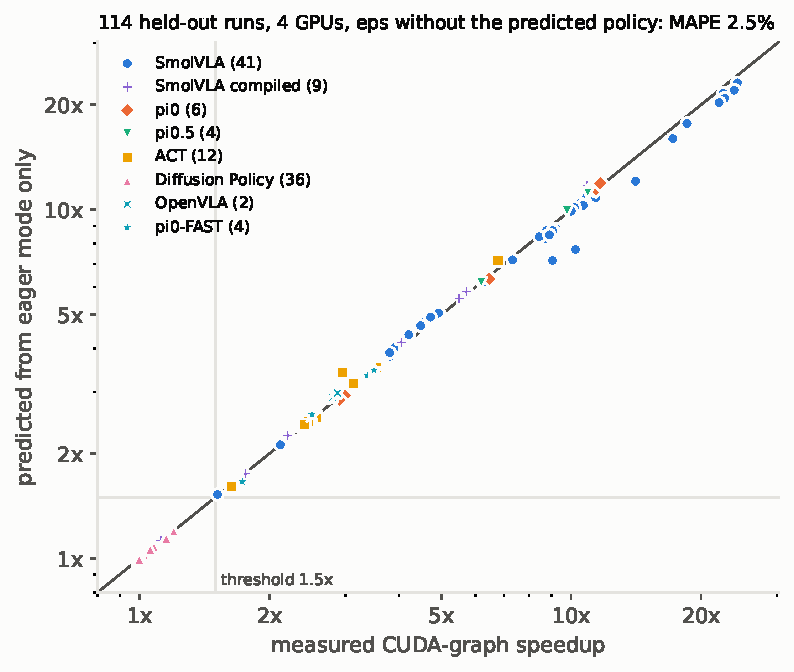
\includegraphics[width=\columnwidth]{figures/graph_worthiness.pdf}
\caption{Graph-worthiness rule: CUDA-graph speedup predicted from eager mode only vs.\ measured,
114 held-out runs on four GPUs, $\varepsilon$ fitted without the predicted policy.}
\label{fig:graphworthiness}
\end{figure}

\begin{figure}[t]
\centering
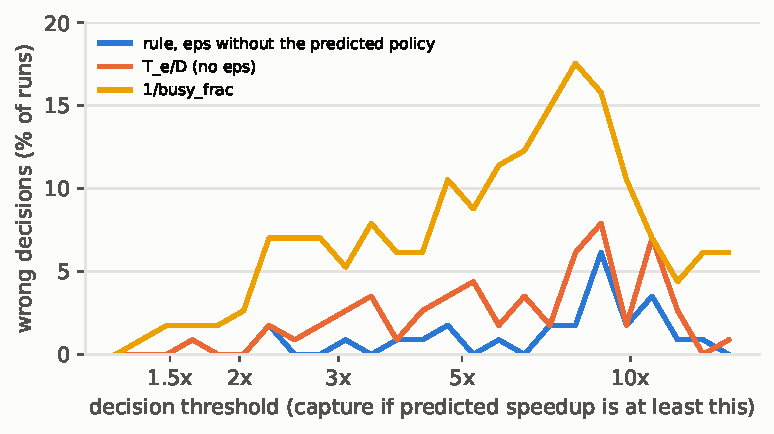
\includegraphics[width=\columnwidth]{figures/graph_worthiness_threshold.pdf}
\caption{Wrong capture decisions as a function of the threshold. Always capturing is wrong for
32 to 93\% of the runs over this range (not shown).}
\label{fig:graphworthiness_threshold}
\end{figure}
 from main.tex (after the cross-GPU
% results). Numbers: results/graph_worthiness.md (model/graph_worthiness.py).
\subsection{When is a CUDA graph worth capturing?}
\label{sec:graphworthiness}

Capturing a region of a PyTorch policy as a CUDA graph is engineering work: buffers must be
static, host synchronizations removed, constant uploads moved out of the region and every input
kept alive. For SmolVLA the vision encoder could not be captured at all (a data dependent
\texttt{arange}), and for OpenVLA the decoder needed a static KV cache and two library patches.
A practitioner therefore wants to know \emph{before} capturing whether the speedup justifies the
work. We give a rule that answers this from eager mode only.

\paragraph{Rule.}
For a candidate region let $T_e$ be its eager wall time, $K$ its number of kernel launches and
$D$ the summed duration of those kernels in one profiled eager step. We predict
\begin{equation}
  \hat T_g = D + K\varepsilon, \qquad \hat S = \frac{T_e}{D + K\varepsilon}
  \approx \frac{c}{t + \varepsilon},
  \label{eq:graphworthiness}
\end{equation}
where $c = T_e/K$ is the eager time per kernel (mostly host dispatch), $t = D/K$ the mean traced
kernel time and $\varepsilon$ the net per-kernel cost of a graph node relative to a traced eager
duration. $\varepsilon$ is the graph node cost minus the profiler's bias on each traced kernel,
so it can be negative. A region is worth capturing when $\hat S$ exceeds a threshold. No graph is
captured to make the prediction.

\paragraph{Evaluation.}
We apply the rule to every run for which we have both an eager kernel trace and a measured graph
time of the same region: SmolVLA (camera, step, chunk, batch and RoboTwin variants), SmolVLA
under \texttt{torch.compile} (fused Triton kernels, eager launches vs.\ compile plus CUDA graph),
$\pi_0$, $\pi_{0.5}$, ACT, Diffusion Policy (default and autotuned cuDNN) and the autoregressive
decoders OpenVLA-7B and $\pi_0$-FAST. That is 114 runs, 95 distinct (configuration, GPU)
situations, 8 policies and 4 GPUs, with measured speedups from 0.99$\times$ to 24.3$\times$. The
SmolVLA baseline configuration, which the fitted variants use, is excluded on every GPU. Repeat
runs make the runs partly dependent, so we also report errors per situation and 95\% confidence
intervals from a bootstrap that resamples configurations. We compare five ways to obtain
$\varepsilon$ that use progressively less information about the predicted run, and two baselines
that need no $\varepsilon$ (Table~\ref{tab:graphworthiness}).

\begin{table*}[t]
\centering
\caption{Error of the predicted CUDA-graph speedup (MAPE over 114 held-out runs, 95\% bootstrap
CI over configurations) and decision accuracy at a 10$\times$ threshold, overall and on the 23
runs whose measured speedup lies within a factor 1.25 of it.}
\label{tab:graphworthiness}
\small
\begin{tabular}{llrrr}
\toprule
Variant & $\varepsilon$ from & MAPE & 95\% CI & 10$\times$ decision (all / hard) \\
\midrule
one $\varepsilon$        & one 2080 Ti run          & 7.1\%  & 4.6--9.9   & 92\% / 61\% \\
$\varepsilon$ per GPU    & one SmolVLA run per GPU  & 1.8\%  & 1.0--2.8   & 98\% / 91\% \\
leave policy out         & other policies, same GPU & 2.5\%  & 1.5--3.8   & 98\% / 91\% \\
leave GPU out            & other GPUs only          & 12.7\% & 8.6--17.1  & 91\% / 57\% \\
\midrule
$T_e/D$ (no $\varepsilon$) & none                   & 7.1\%  & 4.6--9.7   & 98\% / 91\% \\
$1/\text{GPU busy}$      & none (utilization)       & 16.9\% & 11.0--23.7 & 89\% / 57\% \\
\bottomrule
\end{tabular}
\end{table*}

\paragraph{Results.}
With $\varepsilon$ calibrated once per GPU the rule predicts the speedup within 1.8\% on average
(1.9\%, 2.7\%, 1.8\% and 1.1\% on the 2080 Ti, A100, RTX 4070 and TITAN V), and within 2.5\% when
$\varepsilon$ comes only from \emph{other} policies on the same GPU, so a value measured on one
workload transfers to unseen ones, including fused \texttt{torch.compile} kernels (3.1\%) and
autoregressive decoders (OpenVLA 3.6\%, $\pi_0$-FAST 2.1\%). Figure~\ref{fig:graphworthiness}
shows the predictions. The fitted values ($+0.52$, $-0.65$, $-0.35$ and $+0.80\,\mu$s) follow
$\varepsilon = \delta_\text{node} - b$: with the node cost $\delta_\text{node}$ from our C++
calibration and the profiler bias $b$ fitted independently by the cross-GPU model
(Section~\ref{sec:crossgpu}), $\delta_\text{node} - b$ is $+0.43$, $-0.71$ and $+0.69\,\mu$s on
the 2080 Ti, A100 and TITAN V. $\varepsilon$ does not transfer across machines (leave GPU out,
12.7\%) because $b$ is a property of each host's profiler. A utilization counter is a poor
substitute: $1/\text{busy}$ is 16.9\% off and up to 62\% for single runs, because the busy
fraction of a whole step mixes the captured region with the parts that stay eager.

The decision is what a practitioner needs. Most regions are far from a 1.5$\times$ threshold, so
every predictor except the utilization baseline is right for all runs there. We therefore score
decisions at 25 thresholds from 1.2$\times$ to 15$\times$ and separately on the hard runs near
each threshold (Figure~\ref{fig:graphworthiness_threshold}). The leave-policy-out rule is right
for at least 94\% of the runs at every threshold and for 91\% of the hard runs at 5$\times$ and
10$\times$; dropping $\varepsilon$ gives 55\% of the hard runs at 5$\times$, and the utilization
baseline is wrong for up to 18\% of all runs. Within each GPU the predicted speedups order the
regions almost exactly (Spearman $\rho \ge 0.973$).

\paragraph{What sets the speedup.}
Across all eight policies the eager time per kernel $c$ stays between 26 and $44\,\mu$s, while
the mean kernel time $t$ ranges from $3.7\,\mu$s (SmolVLA) to $41\,\mu$s (Diffusion Policy). By
Eq.~\ref{eq:graphworthiness} the speedup is set mainly by $t$: SmolVLA, $\pi_0$ and $\pi_{0.5}$
($t \approx 4$ to $5\,\mu$s) gain up to 24$\times$ at batch 1, ACT, \texttt{torch.compile} and
the decoders ($t \approx 9$ to $13\,\mu$s) 1.1 to 11$\times$, and Diffusion Policy
($t \approx 41\,\mu$s) gains nothing. Batching moves a region along the same curve: SmolVLA's
loop falls from 10$\times$ at batch 1 to 2.1$\times$ at batch 16 on the 2080 Ti as $t$ grows. The same equation explains the eager/graph inversion across GPUs
(Section~\ref{sec:crossgpu}): a slower host raises $c$, a faster GPU lowers $t$, and both raise
the speedup.

\paragraph{How to profile.}
Two measurement rules matter. First, long profiling sessions inflate CUPTI's traced durations on
two of our hosts: a 20-step SmolVLA profile adds about $1\,\mu$s per kernel on the 2080 Ti and A100
hosts and the rule is then 18 to 25\% off, while $K$ and $D$ from a 5-step profile scaled to 20
steps are within 0.2\%. Profile a short window of a periodic loop. Second, profile on a quiet
host. In our host-contention experiment (one core shared with a CPU hog) a profile taken under
contention inflates $t$ from 3.0 to $4.1\,\mu$s and the rule is 19 to 25\% low for SmolVLA, while
$K$ and $D$ from the quiet run with $T_e$ from the contended run are within $+8\%$. ACT stays 27 to
31\% off under two of the three contention modes because its captured region is the whole step,
including host work that contention slows in graph mode too.

\paragraph{Limitations.}
The decoder windows come from the stock dynamic-cache decoder, which launches about 3\% more
kernels per token than the static-cache path that is graphed; OpenVLA has two runs on one GPU.
$\varepsilon$ needs one calibration run per machine. We also measured it without any policy,
with a microbenchmark (\texttt{workloads/eps\_probe.py}: graph time per kernel minus the
CUPTI-traced eager duration on chains of seven small op types at SmolVLA's shapes). On the 2080 Ti
and RTX 4070 it gives $+0.11$ and $-0.05\,\mu$s against $+0.52$ and $-0.35\,\mu$s fitted from
SmolVLA; over the 66 runs on those two GPUs the rule is then 5.2\% off (CI 3.5--7.2\%), better than
no $\varepsilon$ (6.2\%) or one $\varepsilon$ for all GPUs (7.4\%) but well behind one calibration
run of any policy (1.9\% per GPU, 2.4\% leave policy out). The gap differs in sign between the
GPUs, so it is not a constant offset: kernels inside a real policy run with a different cache
state and clock than hot microbenchmark chains, and the RTX 4070 probe ran under a different
PyTorch build (2.8 vs.\ 2.10, so a different CUPTI) than its traces. We therefore recommend
calibrating $\varepsilon$ on one run of a representative policy. The rule predicts the speedup of a region whose kernels stay the same under capture; it
does not predict what fusion would achieve.

\begin{figure}[t]
\centering
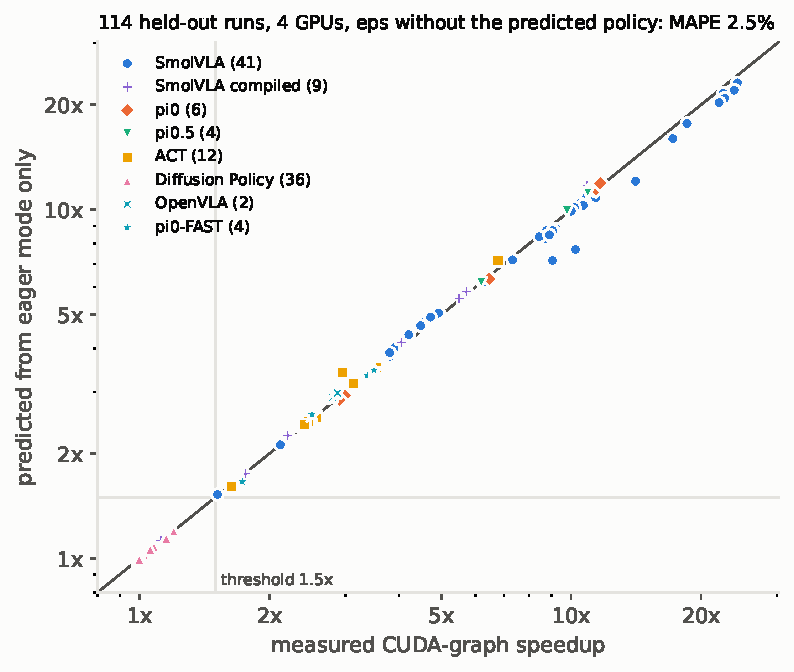
\includegraphics[width=\columnwidth]{figures/graph_worthiness.pdf}
\caption{Graph-worthiness rule: CUDA-graph speedup predicted from eager mode only vs.\ measured,
114 held-out runs on four GPUs, $\varepsilon$ fitted without the predicted policy.}
\label{fig:graphworthiness}
\end{figure}

\begin{figure}[t]
\centering
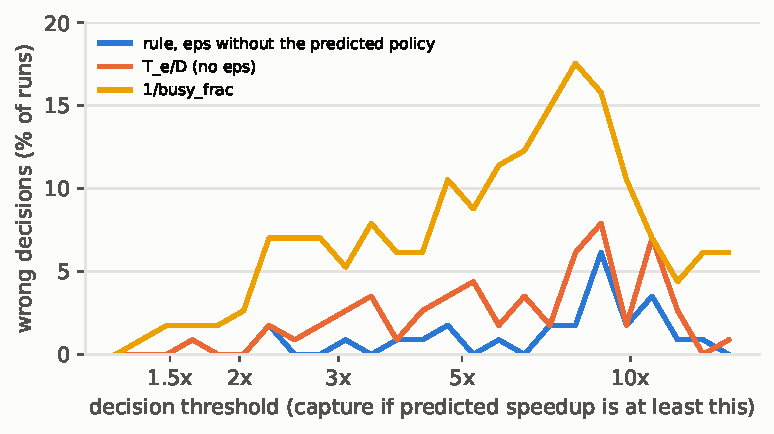
\includegraphics[width=\columnwidth]{figures/graph_worthiness_threshold.pdf}
\caption{Wrong capture decisions as a function of the threshold. Always capturing is wrong for
32 to 93\% of the runs over this range (not shown).}
\label{fig:graphworthiness_threshold}
\end{figure}
